\documentclass [a4paper] {article}
\usepackage[utf8]{inputenc}
\title{Ciencia de datos, práctica 2}
\author{Juan Casado Ballesteros, Samuel García Gonzalez, Iván Anaya Martín}
\usepackage{Sweave}
\begin{document}
\maketitle

\begin{abstract}
Para esta práctica vamos a investigar sobre los algoritmos de asociación.
Utilizaremos apriori para analizar cestas de la compra y datos de vehículos.
Posterioremente explicaremos como funciona el algoritmo de apriori y proporcionaremos un pequeño manual sobre cómo utilizarlo.

Para la parte final aplicaremos el algoritmo apriori sobre conjuntos de datos reales.
También estudiaremos otros algoritmos que calculen la asociación y compararemos sus resultados respecto de los de apriori.
Para estos otros algoritmos haremos también un manual sobre cómo utilizarlos.
\end{abstract}

\newpage
\tableofcontents
\newpage


\section{Asociación sobre los datos de las cestas de la compra}
Hemos introducido los datos de las cestas de la compra en un fichero .txt para evitar tener que escribirlos varias veces.
Utilizamos funciones que hemos creado para automatizar la lectura del fichero y también para utilizar el algoritmo apriori.
En estas funciones solo realizamos una lectura y una ejecición del algoritmo con los parámetros que nosotros hemos elegido.
En el caso del fichero txt guardamos los elementos como listas de la compra en horizonal y los transformamos a como la función que llama a apriori espera recibirlos.
En la función que llama a apriori configuramos como queremos utilizar el algoritmo de modo que no se nos impriman los detalles de su ejecución
ni se calculen las asociaciones con conjuntos vacíos.

\subsection{Cargar los datos de un .txt}
Convierte la matriz a datos booleanos y la transpone, nos es más fácil escribir los datos en horizontal y transponer que no escribirlos ya como se espera que estén.
\begin{Schunk}
\begin{Sinput}
> readAprioriFile
\end{Sinput}
\begin{Soutput}
function(file){
  muestra<-Matrix(as.matrix(read.table(file)), sparse=T)
  muestrangCMatrix<-as(muestra,"nsparseMatrix")
  t(muestrangCMatrix)
}
\end{Soutput}
\end{Schunk}

\subsection{Llamar a apriori}
Con minlen=2 indicamos que no queremos calcular asociaciones con el conjunto vacío y con verbose=F que nos queremos obtener el progreso del algoritmo.
\begin{Schunk}
\begin{Sinput}
> calapriori
\end{Sinput}
\begin{Soutput}
function(matrix,soporte,confianza){
    transacciones<-as(matrix,"transactions")
    asociaciones <- apriori(transacciones, 
        parameter=list(minlen=2, support=soporte,confidence=confianza), 
        control=list(verbose=F))
    inspect(asociaciones)
    asociaciones
}
\end{Soutput}
\end{Schunk}

\subsection{Calcular asociación}
Calculamos la asociación con soporte 0.5 y confianza 0.8 para los datos de las cestas de la compra.

\begin{Schunk}
\begin{Sinput}
> dat = calapriori(readAprioriFile("datos1.txt"),0.5,0.8)
\end{Sinput}
\begin{Soutput}
    lhs             rhs     support   confidence lift count
[1] {Agua}       => {Pan}   0.6666667 1.0        1.20 4    
[2] {Pan}        => {Agua}  0.6666667 0.8        1.20 4    
[3] {Leche}      => {Pan}   0.6666667 0.8        0.96 4    
[4] {Pan}        => {Leche} 0.6666667 0.8        0.96 4    
[5] {Agua,Leche} => {Pan}   0.5000000 1.0        1.20 3    
\end{Soutput}
\end{Schunk}
\begin{center}
\begin{Schunk}
\begin{Sinput}
> plot(dat, method = "two-key plot")
\end{Sinput}
\end{Schunk}
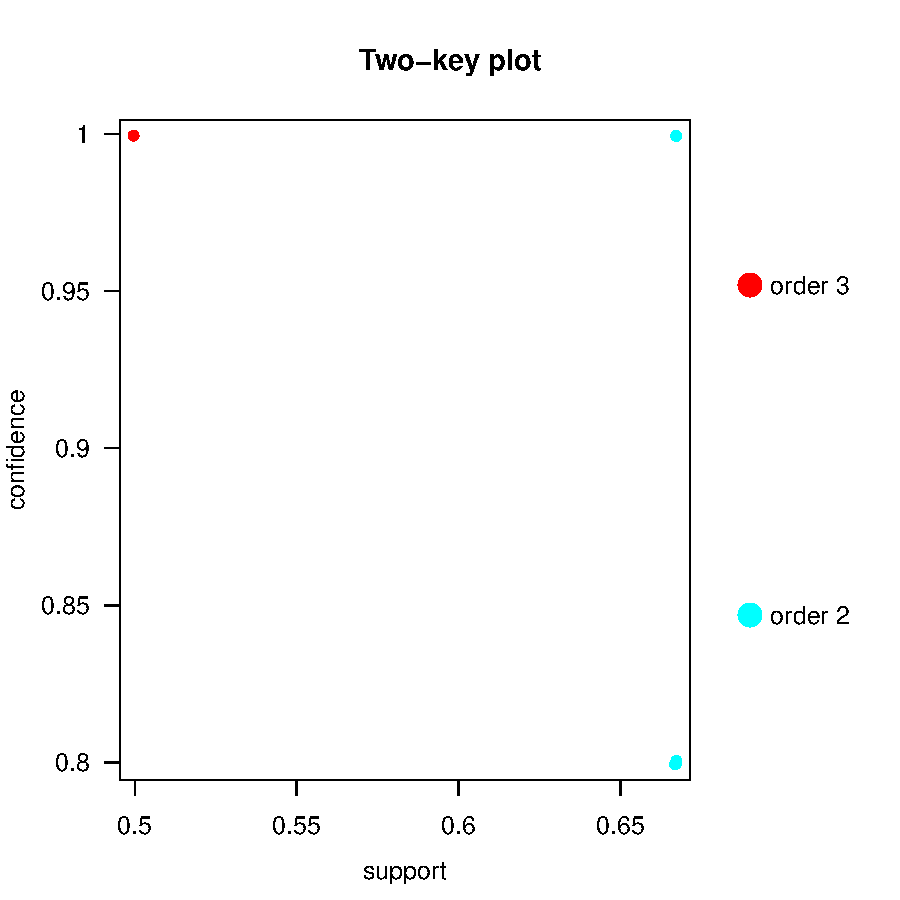
\includegraphics{entrega-grafica_apriori}
\end{center}

\section{Asociación sobre los datos de los vehículos}
Ya habíamos creado las función para leer datos de un .txt y suministrárselos a apriori.
Repetimos el proceso ahora con los datos de los automóbiles iobteniendo los siguentes resultados para un soporte de 0.4 y una confianza de 0.9.


\begin{Schunk}
\begin{Sinput}
> calapriori(readAprioriFile("datos2.txt"),0.4,0.9)
\end{Sinput}
\begin{Soutput}
    lhs                                 rhs              support confidence lift     count
[1] {Control_de_Velocidad}           => {Faros_de_Xenon} 0.625   1          1.333333 5    
[2] {Bluetooth}                      => {Faros_de_Xenon} 0.625   1          1.333333 5    
[3] {Bluetooth,Control_de_Velocidad} => {Faros_de_Xenon} 0.500   1          1.333333 4    
set of 3 rules 
\end{Soutput}
\end{Schunk}

\section{Qué es apriori y cómo utilizarlo}
El algoritmo a priori surge como respuesta al problema existente a la hora de analizar las reglas de asociación 
entre diferentes datos, puesto que con unas decenas de datos diferentes podemos encontrar miles de reglas diferentes y el
principio en el que se basa es que si un conjunto de datos es frecuente, cualquier subconjunto del mismo también lo será. 
Este algoritmo encuentra reglas de asociación entre diferentes datos en base a dos parámetros que establecemos 
arbitrariamente que tienen que cumplirse en ellas, que son el soporte y la confianza. El soporte de un conjunto de datos se 
define como la proporción de apariciones que contiene dicho conjunto de datos en el espacio muestral. La confianza define 
la probabilidad de encontrar relacionadas una parte derecha de una regla de asociación con una parte izquierda determinadas.

\vspace{5mm}

Invocamos la función escribiendo apriori() y los diferentes parámetros que nos interesan para su uso son los siguientes:
Apriori(data, parameter = NULL, appearance = NULL, control = NULL)
Data: estructura de datos (por ejemplo, una matriz binaria o un data.frame) que se puede convertir en transacciones.
Parameter: diferentes parámetros de la clase APparameter. El comportamiento por defecto de los parámetros importantes es: soporte (support) de 10%, confianza (confidence) del 80% un límite máximo (maxlen) de 10 y mínimo (minlen) de 1 elemento por conjunto de elementos, teniendo en cuenta el conjunto vacio y un tiempo de check (maxtime) máximo de 5 segundos.
Appearance: diferentes parámetros de la clase APappearance. Con esto podemos restringir la aparición de algunos datos.
Control: diferentes parámetros de la clase APcontrol. Controla el rendimiento del algoritmo (sort, heap, filter…) y aspectos como la ordenación o el reporte del rendimiento (verbose).

\section{Creación de un algoritmo apriori}
Hemos programado una versión simplificada del algoritmo eliminando algunas de las optimizaciones que este realiza.
La funcionalidad de nuestro algoritmo también es reducida y solo está pensado para tomar como entrada tablas de datos booleanos 
a diferencia del apriori original que puede tomar otros tipos de dato como entrada.
Para implementarlo lo hemos hecho utilizando tres funciones.

Repetimos el cálculo de la asociación para los datos de las cestas de la compra y de los automóbiles comprobando que nuestro algoritmo proporciona
los mismos resultados que apriori nos había dado anteriormente. Comprobamos que el algoritmo se comporta como esperábamos.
\begin{Schunk}
\begin{Sinput}
> print(toTable(f_apriori(readAprioriFile("datos1.txt"),0.5,0.8)),right=F)
\end{Sinput}
\begin{Soutput}
  lhs             rhs     support   confidence lift count
1 {Pan}        => {Agua}  0.6666667 0.8        1.20 4    
2 {Agua}       => {Pan}   0.6666667 1.0        1.20 4    
3 {Pan}        => {Leche} 0.6666667 0.8        0.96 4    
4 {Leche}      => {Pan}   0.6666667 0.8        0.96 4    
5 {Agua,Leche} => {Pan}   0.5000000 1.0        1.20 3    
\end{Soutput}
\begin{Sinput}
> print(toTable(f_apriori(readAprioriFile("datos2.txt"),0.4,0.9)),right=F)
\end{Sinput}
\begin{Soutput}
  lhs                                 rhs              support confidence lift     count
1 {Bluetooth}                      => {Faros_de_Xenon} 0.625   1          1.333333 5    
2 {Control_de_Velocidad}           => {Faros_de_Xenon} 0.625   1          1.333333 5    
3 {Bluetooth,Control_de_Velocidad} => {Faros_de_Xenon} 0.500   1          1.333333 4    
\end{Soutput}
\end{Schunk}

\section{Apriori sobre un dataset real}
Buscando informcación sobre el algoritmo apriori y sobre otros algoritmos de asociación hemos encontrado distintas fuentes de las que obtener datos típicos 
sobre los que aplicar algoritmos de asociación.
Hemos elegido un conjunto de datos que están ya incluidos en el paquete arules para probar sobre ellos el comportamiento del algoritmo.

Podemos observar que la asociación puede aplicarse también sobre variables con múltiples valores, no solo verdadero o falso.
Los datos contienen 8993 observaciones en 14 variables. El primer paso para procesarlos es crear clases de equivalencia (2) para cada valor.
Una vez hecho esto solo nos queda crear las transacciones y proporcionárselas al algoritmo apriori.

\begin{Schunk}
\begin{Sinput}
> data("IncomeESL")
> IncomeESL[1:3, ]
\end{Sinput}
\begin{Soutput}
  income    sex marital status   age           education              occupation years in bay area
1    75+ female        married 45-54 college (1-3 years)               homemaker               >10
2    75+   male        married 45-54    college graduate               homemaker               >10
3    75+ female        married 25-34    college graduate professional/managerial               >10
  dual incomes number in household number of children householder status type of home
1           no                   3                  0                own        house
2           no                   5                  2                own        house
3          yes                   3                  1               rent    apartment
  ethnic classification language in home
1                 white             <NA>
2                 white          english
3                 white          english
\end{Soutput}
\begin{Sinput}
> IncomeESL <- IncomeESL[complete.cases(IncomeESL), ]
> IncomeESL[["income"]] <- factor((as.numeric(IncomeESL[["income"]]) > 6) +1,
+   levels = 1 : 2 , labels = c("$0-$40,000", "$40,000+"))
> IncomeESL[["age"]] <- factor((as.numeric(IncomeESL[["age"]]) > 3) +1,
+   levels = 1 : 2 , labels = c("14-34", "35+"))
> IncomeESL[["education"]] <- factor((as.numeric(IncomeESL[["education"]]) > 4) +1,
+   levels = 1 : 2 , labels = c("no college graduate", "college graduate"))
> IncomeESL[["years in bay area"]] <- factor(
+   (as.numeric(IncomeESL[["years in bay area"]]) > 4) +1,
+   levels = 1 : 2 , labels = c("1-9", "10+"))
> IncomeESL[["number in household"]] <- factor(
+   (as.numeric(IncomeESL[["number in household"]]) > 3) +1,
+   levels = 1 : 2 , labels = c("1", "2+"))
> IncomeESL[["number of children"]] <- factor(
+   (as.numeric(IncomeESL[["number of children"]]) > 1) +0,
+   levels = 0 : 1 , labels = c("0", "1+"))
> calapriori(IncomeESL, 0.5,0.9)
\end{Sinput}
\begin{Soutput}
    lhs                              rhs                          support confidence     lift count
[1] {sex=female}                  => {language in home=english} 0.5122164  0.9246521 1.012890  3522
[2] {type of home=house}          => {language in home=english} 0.5446481  0.9129693 1.000092  3745
[3] {dual incomes=not married}    => {language in home=english} 0.5426120  0.9069033 0.993447  3731
[4] {number of children=0}        => {language in home=english} 0.5801338  0.9328812 1.021904  3989
[5] {years in bay area=10+}       => {language in home=english} 0.6013671  0.9300495 1.018802  4135
[6] {ethnic classification=white} => {language in home=english} 0.6595404  0.9847991 1.078776  4535
[7] {number in household=1}       => {language in home=english} 0.6495055  0.9388270 1.028417  4466
[8] {number in household=1,                                                                        
     number of children=0}        => {language in home=english} 0.5213787  0.9424290 1.032363  3585
set of 8 rules 
\end{Soutput}
\end{Schunk}


\section{Otros algoritmos de asociación}

\subsection{Que es eclat y cómo utilizarlo}
Eclat es una alternativa a apriori que utiliza para cada elemento una lista en la que se registra en qué transacción está el 
elemento mencionado, reduciendo así enormemente el tiempo de cómputo, pero aumentando el consumo de memoria. La idea básica 
es que usa estas listas y realiza intersecciones con otras para calcular el soporte del elemento, evitando generar subconjuntos 
que no existan en el espacio muestral.

Invocamos la función escribiendo eclat() y los diferentes parámetros que nos interesan para su uso son los siguientes:
Eclat(data, parameter = NULL,  control = NULL)
Data: estructura de datos (por ejemplo, una matriz binaria o un data.frame) que se puede convertir en transacciones.
Parameter: diferentes parámetros de la clase ECparameter. El comportamiento por defecto de los parámetros importantes es: soporte (support) de 10% y un límite (maxlen) de 5 elementos por conjunto de elementos.
Control: diferentes parámetros de la clase ECcontrol. Controla el rendimiento del algoritmo (sort, heap, filter…) y aspectos como la ordenación o el reporte del rendimiento (verbose).

\subsubsection{Ejemplos de con eclat}
Ejecución sobre la muestra de los datos de las cestas de la compra.
\begin{Schunk}
\begin{Sinput}
> caleclat(readAprioriFile("datos1.txt"),0.5)
\end{Sinput}
\begin{Soutput}
    items            support   count
[1] {Pan,Agua,Leche} 0.5000000 3    
[2] {Pan,Agua}       0.6666667 4    
[3] {Agua,Leche}     0.5000000 3    
[4] {Pan,Leche}      0.6666667 4    
set of 4 itemsets 
\end{Soutput}
\end{Schunk}

Ejecución sobre la muestra de los datos de los componentes de los coches.
\begin{Schunk}
\begin{Sinput}
> caleclat(readAprioriFile("datos2.txt"),0.4)
\end{Sinput}
\begin{Soutput}
    items                                           support count
[1] {Faros_de_Xenon,Bluetooth,Control_de_Velocidad} 0.500   4    
[2] {Faros_de_Xenon,Control_de_Velocidad}           0.625   5    
[3] {Bluetooth,Control_de_Velocidad}                0.500   4    
[4] {Faros_de_Xenon,Bluetooth}                      0.625   5    
set of 4 itemsets 
\end{Soutput}
\end{Schunk}

Ejecución sobre la muestra de los datos demográficos incluídos en el paquete arules.
\begin{Schunk}
\begin{Sinput}
> caleclat(IncomeESL, 0.5)
\end{Sinput}
\begin{Soutput}
     items                             support count
[1]  {sex=female,                                   
      language in home=english}      0.5122164  3522
[2]  {age=14-34,                                    
      language in home=english}      0.5248691  3609
[3]  {type of home=house,                           
      language in home=english}      0.5446481  3745
[4]  {dual incomes=not married,                     
      language in home=english}      0.5426120  3731
[5]  {number in household=1,                        
      number of children=0,                         
      language in home=english}      0.5213787  3585
[6]  {number of children=0,                         
      language in home=english}      0.5801338  3989
[7]  {number in household=1,                        
      number of children=0}          0.5532286  3804
[8]  {income=$0-$40,000,                            
      language in home=english}      0.5578825  3836
[9]  {income=$0-$40,000,                            
      education=no college graduate} 0.5018906  3451
[10] {years in bay area=10+,                        
      language in home=english}      0.6013671  4135
[11] {ethnic classification=white,                  
      language in home=english}      0.6595404  4535
[12] {number in household=1,                        
      ethnic classification=white}   0.5001454  3439
[13] {number in household=1,                        
      language in home=english}      0.6495055  4466
[14] {education=no college graduate,                
      language in home=english}      0.6343805  4362
set of 14 itemsets 
\end{Soutput}
\end{Schunk}

Podemos observar que obtenemos el mismo soporte que con apriori y que tal y como hemos dicho la confianza no es calculada.
Para compara los resultados de apriori con los de eclat debemos buscar en apriori los conjuntos que se correspondan con los de eclar.

Ej: los conjuntos de apriori: {Pan} => {Agua} y {Agua} => {Pan} en eclat serán solo uno: {Pan, Agua}

\end{document}
